\documentclass[pdflatex,a4paper,11pt,titlepage]{article}

%% Load packages ========================================
\usepackage[T1]{fontenc}

%\usepackage{xr-hyper} % needs to be loaded before hyperref
\usepackage{ifpdf,ifxetex}
\ifxetex
  \usepackage{epstopdf}
  \epstopdfsetup{suffix=.\SourceExt}
  \usepackage{fontspec}           % XeLaTeX specific
  \defaultfontfeatures{Mapping=tex-text} % For archaic input (e.g. convert -- to en-dash)
  \setmainfont{Linux Libertine O}  % LaTeX default (Computer Modern Unicode)
  \usepackage[xetex,colorlinks,unicode=True]{hyperref}
\else
  \usepackage[utf8]{inputenc}     % support utf8 (if possible: use xetex)
  \usepackage{lmodern}
  \usepackage{newunicodechar}
  \ifpdf
    \usepackage[pdftex]{graphicx}
    \usepackage{epstopdf}
    \epstopdfsetup{suffix=.\SourceExt}
    \usepackage[pdftex,colorlinks,unicode=True]{hyperref}
  \else
    \usepackage{graphicx}
    \usepackage[colorlinks,unicode=True]{hyperref}
  \fi
\fi
\usepackage[dvipsnames]{xcolor}
\usepackage{subfig}

\usepackage{booktabs} % <--- This is the way to do it if you ask me.

\usepackage[absolute,overlay]{textpos} % textblock (see inc/kth_titlepage)

\usepackage{authblk}
\renewcommand\Authsep{, }
\renewcommand\Authand{ och }
\renewcommand\Authands{, och }
%\renewcommand*{\thefootnote}{\fnsymbol{footnote}}
\usepackage[perpage]{footmisc} % \cite => numbers
\renewcommand{\thefootnote}{\fnsymbol{footnote}}
\usepackage[style=chem-acs,doi,autocite=superscript,pageranges=false,backend=biber]{biblatex}
\AtEveryBibitem{\clearfield{month}} % Don't put "Jan. 2000" in references
\AtEveryCitekey{\clearfield{month}} % http://tex.stackexchange.com/questions/55780
\renewcommand{\cite}{\autocite}
\usepackage{amsmath, amsfonts, amssymb, amsthm}
\usepackage{siunitx}
\DeclareSIUnit\molar{\mole\per\cubic\deci\metre}
\DeclareSIUnit\Molar{\textsc{m}}
\usepackage[version=3]{mhchem}
%\usepackage{chemstyle}  % \standardstate symbol
\newcommand*{\plimsoll}{{\ensuremath{-\kern-5pt{\circ}\kern-5pt-}}} % standard state symbol

% Make References appear in Table of Contents
\usepackage[nottoc,notlof,notlot,numbib]{tocbibind}

\hypersetup{%
  bookmarksnumbered=true, %
  breaklinks=false, %
  raiselinks=true, %
  pdfborder={0 0 0}, %
  colorlinks=true, %
  plainpages=false, %
  pdfstartview={FitH}, %
  pdfcreator={LaTeX with hyperref package}, %
  citecolor=teal, % See xcolor package documentation
  linkcolor=Maroon, %
  urlcolor=blue, %
}%

\usepackage{minted}

% Minted matlab code
\definecolor{mintedbackground}{rgb}{0.95,0.95,0.95}

\newmintedfile[matlabcode]{matlab}{
bgcolor=mintedbackground,
fontfamily=tt,
fontsize=\footnotesize,
linenos=true,
numberblanklines=true,
numbersep=12pt,
numbersep=5pt,
gobble=0,
frame=leftline,
framerule=0.4pt,
framesep=2mm,
funcnamehighlighting=true,
tabsize=4,
obeytabs=false,
mathescape=false
samepage=false, %with this setting you can force the list to appear on the same page
showspaces=false,
showtabs =false,
texcl=false,
}
%% Global Last Commands
\usepackage[capitalise,noabbrev,swedish]{cleveref} % <--- Needs to be loaded late (see doc)
\usepackage{listings}

\lstnewenvironment{terminaloutput}{%
  \lstset{backgroundcolor=\color{mintedbackground},
  frame=single,
  breaklines=true,
  framerule=0pt,
  basicstyle=\footnotesize\ttfamily,
  columns=fullflexible}}{}

\renewcommand{\thesection}{B\arabic{section}} % Bilaga

\providecommand{\projecttitle}{Stopped flow - Bilaga}
\hypersetup{%
  pdfkeywords={stopped flow},%
  pdfauthor={Björn Dahlgren},%
  pdftitle={KD1080 \projecttitle}%
}
\providecommand{\mailto}{\texttt{\href{mailto:bda@kth.se}{bda@kth.se}}}
\author[1]{Björn Dahlgren (\mailto)}
\affil[1]{School of Chemical Science and Engineering, Applied Physical Chemistry, KTH}

\title{\projecttitle}


\begin{document}
 
  \begin{titlepage}
    \maketitle
  \end{titlepage}
  \tableofcontents
  \listoffigures
  %\listoftables
  \pagebreak

  \setlength{\parindent}{0em}
  \setlength{\parskip}{1em}


  \section{Exempelskript för ickelinjär kurvanpassning}
\label{sec:matlab-nonlinear}
Nedan finner ni ett Matlab skript ({\tt passning.m}) för incke linjär kurvanpassning.
Ekvationen som passas i exemplet är helt godtycklig:

\begin{equation}
  \label{eq:ex}
  f(x) = a\frac{x^b+1}{x^{b+1}+1}
\end{equation}

Vi genererar data för passning med brus och låter Matlabs funktion
``fit'' optimera $a$ och $b$ (se \cref{fig:matlab-nonlinear}).

\begin{figure}
  \centering
  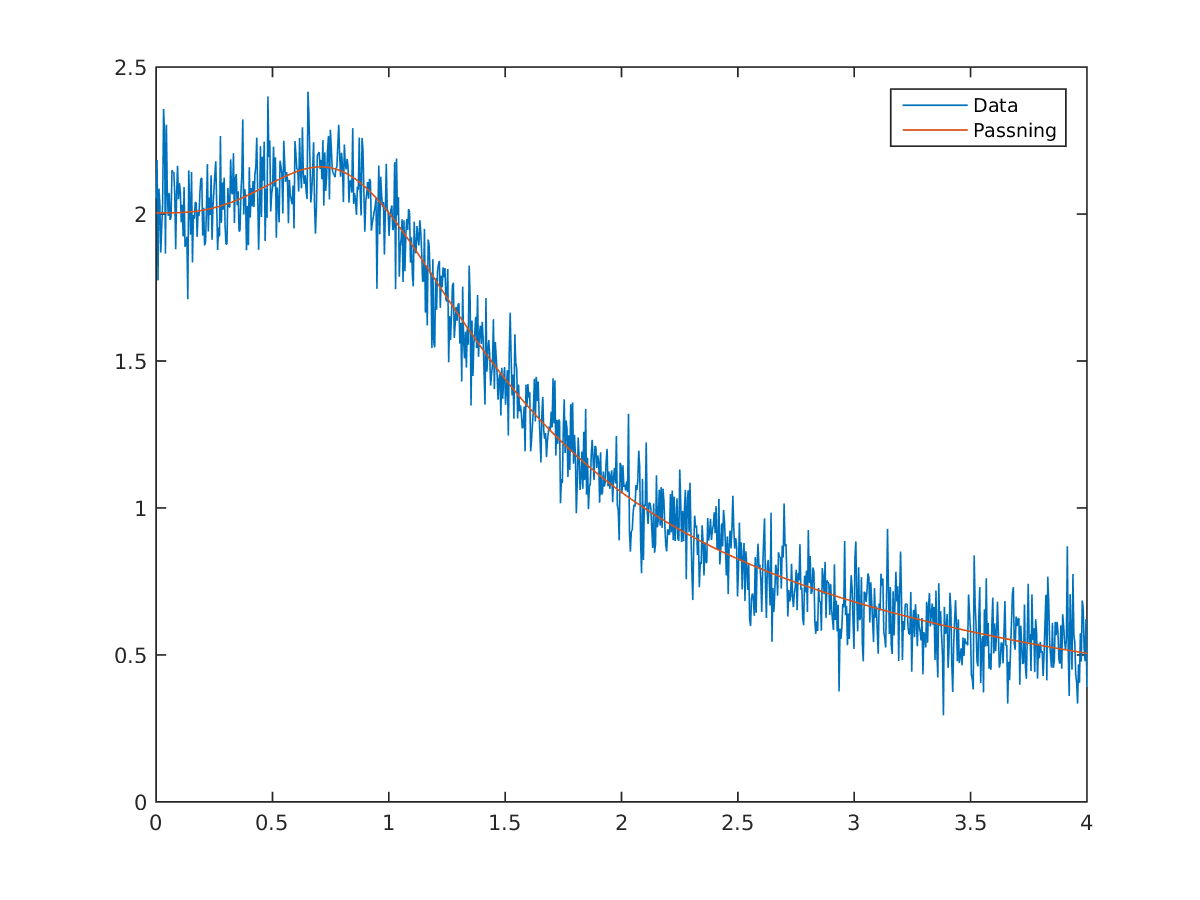
\includegraphics[scale=0.5]{matlab/passning.png}
  \caption{Ickelinjär kurvanpassning}
  \label{fig:matlab-nonlinear}
\end{figure}

\matlabcode{matlab/passning.m}

När vi exekverar koden ovan får vi följande utdata i terminalen:

\begin{terminaloutput}
>> passning

fitobj = 

     General model:
     fitobj(x) = (a*g(b,x)./g(b+1,x))
     Coefficients (with 95% confidence bounds):
       a =       2.004  (1.988, 2.02)
       b =       3.207  (2.813, 3.601)

standard_deviation =

    0.0082    0.2009


root_mean_square_error =

    0.0999
\end{terminaloutput}

Vi ser att passningen lyckades och de sanna värdena ligger väl inom
angivna 95\%  konfidensintervall. Vi noterar dock att osäkerheten är
relativt stor för {\tt b}. Observera att vi gav startvärdena 1 för
optimeringen av $a$ och $b$. För att kurvanpassningen skall vara pålitlig
bör man försöka välja så bra startvärden som möjligt. Genom att titta på
den brusiga kurvan i \cref{fig:matlab-nonlinear} kunde vi t. ex. från
skärningspunkten med y-axeln satt startgissningen för $a$ någonstans
kring 2 och sedan löst ut $b$ ur en approximativ version av \cref{eq:ex} för
$f(4) \approx 0.5$.

Ett alternativ till att använda funktionen {\tt fit} är att använda {\tt
  fsolve} vilket kan ansättas att försöka lösa en ekvation för
residualerna för vår passning:

\matlabcode{matlab/passning2.m}

\begin{terminaloutput}
>> passning2
Warning: Trust-region-dogleg algorithm of FSOLVE cannot handle non-square systems; using Levenberg-Marquardt algorithm instead. 
> In fsolve (line 287)
  In passning2 (line 43) 

No solution found.

fsolve stopped because the last step was ineffective. However, the vector of function
values is not near zero, as measured by the default value of the function tolerance. 

<stopping criteria details>


result =

    2.0015    2.9760
\end{terminaloutput}

metoden med {\tt fsolve} producerar likvärdiga passningar men ger
inga konfidensintervall, samt varnar för det mesta (om inställningar inte
görs aktivt) att efterfrågade toleranser inte kunde uppnås. Använd den
metod ni är mest bekväma med: antingen {\tt fsolve} eller {\tt fit}.

%%% Local Variables:
%%% mode: latex
%%% TeX-master: "../main"
%%% ispell-local-dictionary: "swedish"
%%% End:

  \section{Exempelskript för viktad minsta-kvadrat anpassning}
\label{sec:matlab-wls}
Nedan finner ni ett Matlab skript ({\tt wls.m}) för viktad
minsta-kvadrat anspassning av en rät linje till en serie punkter med
uppskattad osäkerhet för varje separat punkt.

\matlabcode{matlab/wls.m}

\begin{terminaloutput}
>> wls

k =

    3.1619


m =

    2.6406


dk =

    0.2415


dm =

    1.1118
\end{terminaloutput}

Notera att vi även tog fram nya felgränser (en standardavvikelse vilket
motsvarar ett 68.27\% konfidensintervall) på våra två
parametrar. \cref{fig:matlab-wls} visar den genererade plotten.

\begin{figure}
  \centering
  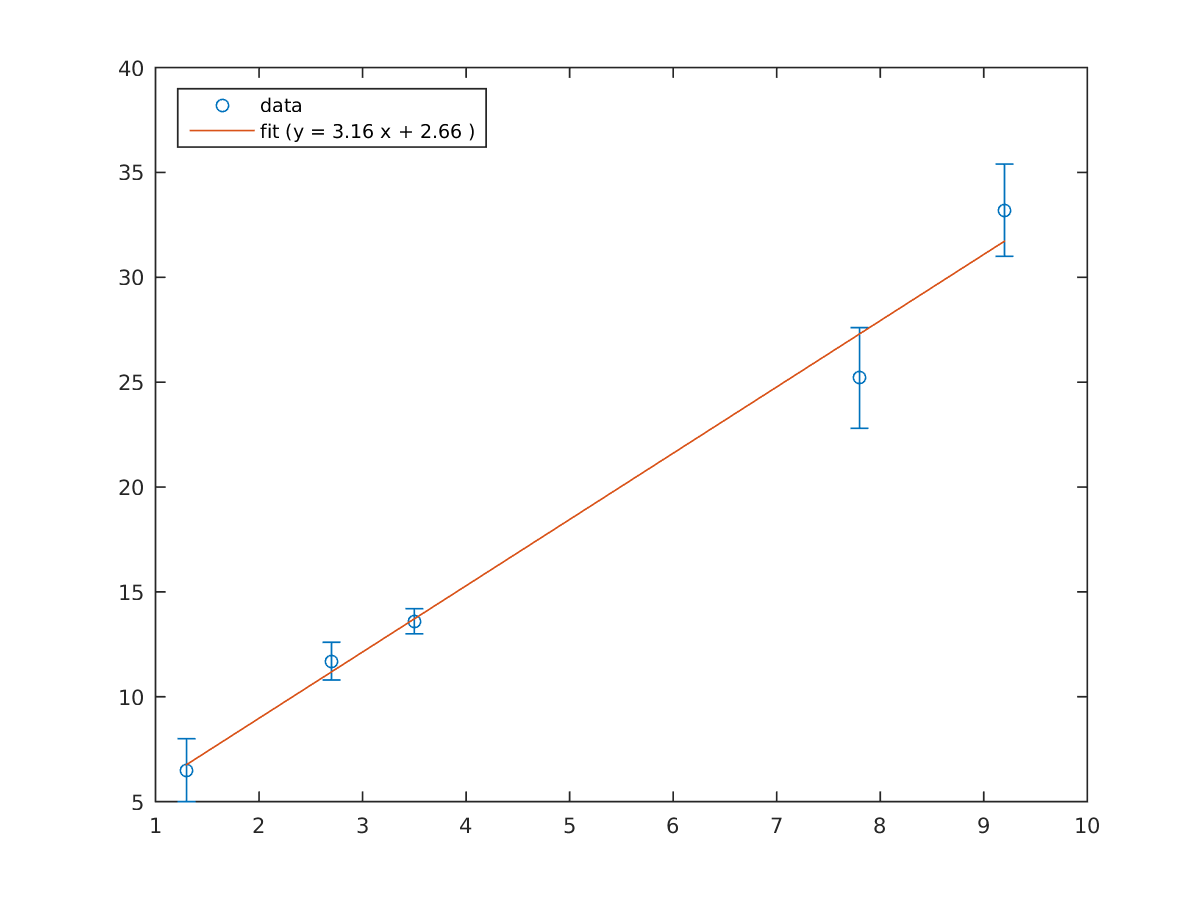
\includegraphics[scale=0.5]{matlab/wls_fit.png}
  \caption{Viktad minsta-kvadrat anpassning}
  \label{fig:matlab-wls}
\end{figure}

%%% Local Variables:
%%% mode: latex
%%% TeX-master: "../main"
%%% ispell-local-dictionary: "swedish"
%%% End:

  \section{Exempelskript för automatisk passning av flera datafiler}
\label{sec:matlab-loop-read-fit}
Detta exempel förutsätter följande mappstruktur:

\begin{terminaloutput}
.
+-- 15
|   +-- 1.txt
|   +-- 2.txt
+-- 19
|   +-- 1.txt
|   +-- 2.txt
+-- anpassa.m
+-- anpassa_alla.m
\end{terminaloutput}

Nedan finner ni ett Matlab skript ({\tt anpassa\_alla.m}), som
i en dubbel-loop anropar en egenskriven passningsfunktion ({\tt
  anpassa.m}) som gör en linjär regression för en specifierad textfil. 

\matlabcode{matlab/anpassa_alla.m}

\begin{terminaloutput}
>> run anpassa_alla
    15

     1

    1.9329    0.2377    0.1234    0.3236

     2

    1.8325    0.2961    0.1762    0.6239

    19

     1

    2.9699    0.2328    0.7338    1.7560

     2

    3.0746   -0.1011    0.0531    0.2119
\end{terminaloutput}

Funktionen som utför passningen ({\tt anpassa.m}) ser ut enligt följande:

\matlabcode{matlab/anpassa.m}

%%% Local Variables:
%%% mode: latex
%%% TeX-master: "../main"
%%% ispell-local-dictionary: "swedish"
%%% End:


\end{document}
